\chapter{对抗生成网络在人脸属性中的应用}
\section{对抗生成网络相关技术的介绍}
早在2014年,人们对于神经网络技术的研究非常狂热的同时,也有一部分理智的科学家认为神经网络的输出判断具有非常高的风险,输出具有非常高的不稳定性,所谓数据集上的准确率超越人类不过是一场谎言,为了戳穿这一谎言,他们在神经网络判断正确的图片上简单加了一些噪声,对于人类来说根本没有察觉图像的变化,但是在神经网络却完全将其判断成另外一种物体。同时科学家们宣称这样极具欺骗性的图片并非偶然得到,而是可以量产的,比如通过对抗生成网络。

借助于博弈论中的零和博弈思想(在零和博弈中,游戏玩家之间的利益总和是固定的,即一方获得收益,另一方就要承担损失。)Goodfellow极具想象力的提出了可以通过搭建两个对抗的网络,各自的目的就是降低对方的准确率,或者说提升对方loss。通过这样非常具有竞争性的训练过程,最够提升两个网络的性能。具体来讲:在对抗生成网络中,玩家的角色会分别有生成模型(generative model)和判别式模型(discriminative model)充当.生成模型G捕捉样本数据的分布,判别模型D是一个二分类器,估计一个样本来自于训练数据(而非生成数据)的概率。G和D可以是线性代数的算法操作组合,也可以是神经网络的网络模型,都可以理解成或者定义成非线性函数。通过不断调整G和D,直到D不能把事件区分出来为止。在调整过程中,一方面需要优化G,使得它尽可能的让D混淆;另一方面需要优化D,使得它尽可能的能区分出假冒的东西;当D无法区分出事件的来源的时候,可以认为,G和M是一样的。从而,就获得了能够以假乱真的数据。

但是对抗生成网络很明显并不能像正常的CNN网络一样对于具体的模式识别任务,但是作为探究CNN生成原理的一部分,对抗生成网络主要是希望能够了解CNN能够从图像中学习到什么样的信息,怎样学习的,并且能否以较为直观的形式也就是生成图像来表示出来,(尽管学习到的东西很多时候并不能够以图像的形式进行展现)。
\section{探究对抗神经网络的应用}
在之前对于对抗生成网络的介绍中,可以发现对抗生成网络最初是来证明神经网络算法对于数据分布具有一定的局限性。而慢慢发展,人们并不在乎神经网络是否对于数据分布有一定的的局限性,而狂热的希望能够通过对抗生成网络获得以假乱真的机器生成图片。似乎人们觉得如果机器能创造他,那机器肯定可以了解他,那么识别他也是轻而易举。于是乎这种炫酷,但是有一定投机取巧性质的思路不仅开始影响最初使用对抗生成网络探究神经网络有效性的本意,也影响着各种识别任务的传统数据+模型的预测方式。

在现有基于模型和分类算法的场景下,对抗神经网络还很难展现出对于属性任务有明显的提升,而对抗生成网络往往以生成各种图片来获得关注和人们的注意,而在业内确实有一些方法可以生成带有人脸属性的人脸图片。那么是否可以通过生成图片的方式为神经网络增加训练的数据,从而起到为属性识别增添数据的作用就成了对抗生成网络在人脸属性上的应用方向。首先可以从使用对抗生成网络直接生成训练数据的方向入手。
\subsection{使用对抗生成网络生成真实图像}
首先参考了DCGAN\cite{DCGAN}的方法和思路,采用了如下的网络结构作为生成图像的基本架构, 生成模型:输入100维的噪声到第一个全连接层,将其映射为1024维,然后再把1024的一维向量重塑成1024个通道的4x4的特征图。基本规律是生成网络的每一个下一层是反卷积层,通道数减半,图像尺寸加倍。

判别模型:就是一个没有池化层的全卷积网络,输入是生成模型输出的图像,输出一个标量,表示输入数据属于训练数据而非生成样本的概率。
\begin{figure}[h]
  \centering
  \subfigure{
  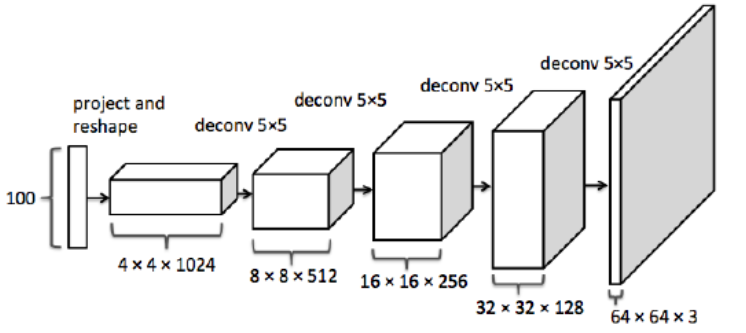
\includegraphics[width=3.0in]{DCGAN_g.png}
  }
  \subfigure{
  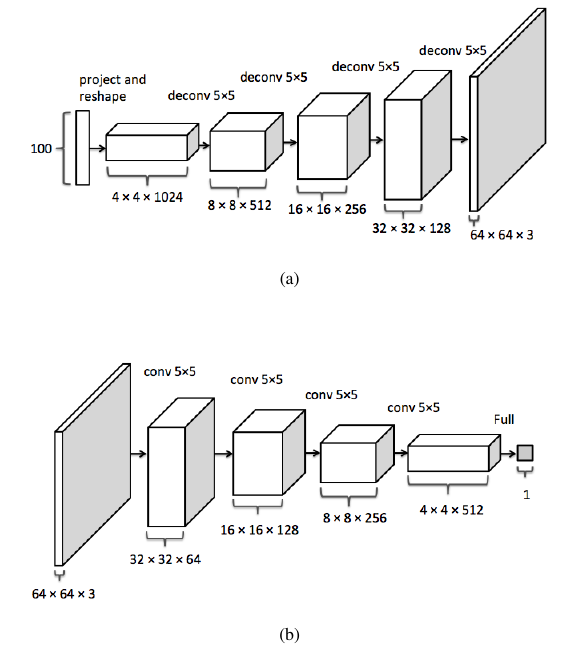
\includegraphics[width=3.0in]{DCGAN_d.png}
  }
  \caption{DCGAN的网络结构:(a)DCGAN中的生成网络模型结构;(b)DCGAN中的判决模型网络结构}
\end{figure}

\subsubsection{生成数字图像}
首先使用mnist数据\cite{MNIST}作为训练样本,实现了从100维的噪声生成数字图像,发现对抗生成网络确实可以生成较为逼真的数字图片,而且生成的图片并不局限于一种状态。
\begin{figure}[!ht]
 \centering 
	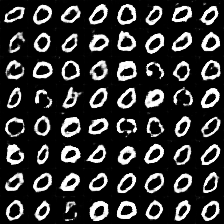
\includegraphics[width=1.0in,height=1.0in]{minnum0.png}
	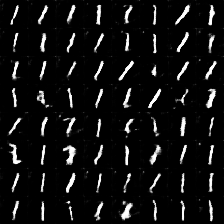
\includegraphics[width=1.0in,height=1.0in]{minnum1.png}
	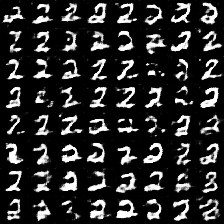
\includegraphics[width=1.0in,height=1.0in]{minnum2.png}
	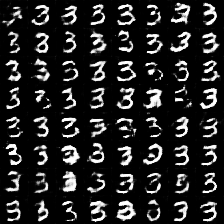
\includegraphics[width=1.0in,height=1.0in]{minnum3.png}
	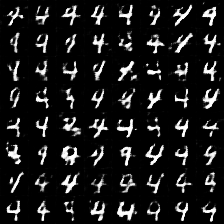
\includegraphics[width=1.0in,height=1.0in]{minnum4.png}
	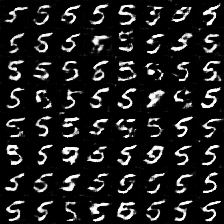
\includegraphics[width=1.0in,height=1.0in]{minnum5.png}
	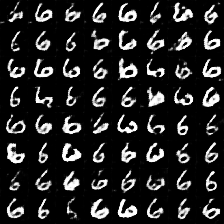
\includegraphics[width=1.0in,height=1.0in]{minnum6.png}
	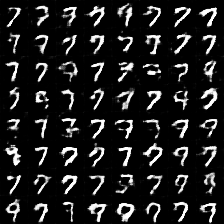
\includegraphics[width=1.0in,height=1.0in]{minnum7.png}
	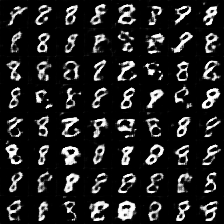
\includegraphics[width=1.0in,height=1.0in]{minnum8.png}
	\caption{minist图片生成的数字图片}
\end{figure}

\subsubsection{生成物体图像}
于是,我们加大了训练的难度,更换cifar10\cite{CIFAR10}数据作为训练的样本,实现了32*32的彩色物体图像生成,但是发现效果似乎并不够出色,在生成的的过程中,虽然能够看物体的生成具有一定的个形状信息和物体轮廓,但是整体的效果却不是很好,不能够生成出具体的能够和真是图像匹配的物体图片。
\begin{figure}[!ht]
 \centering 
	\subfigure[真实的cifar10图像数据]{
	\includegraphics[width=2.0in,height=2.0in]{realGAN.png}
	}
	\subfigure[伪造的cifar10图像数据]{
	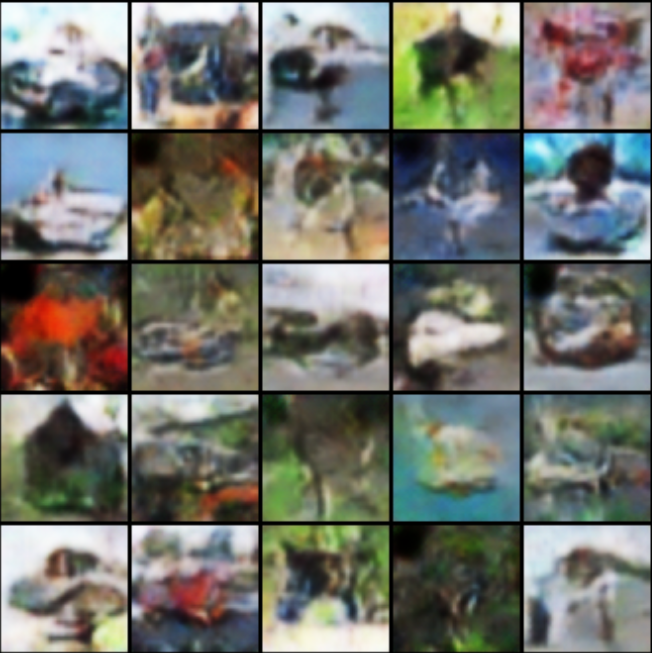
\includegraphics[width=2.0in,height=2.0in]{fake.png}
	}
	\caption{cifar10图片生成的数字图片}
\end{figure}

\subsubsection{生成人脸图像}
那么任务换到在人脸图片的生成上,我们决定放弃DCGAN的结构,装用BGAN\cite{BGAN}和WGAN距离\cite{WGAN}的方式进行人脸图像的生成,事实证明相比于DCGAN,这种方式可以取得更加鲁棒和逼真的效果。

WGAN:

\begin{figure}
  \centering
    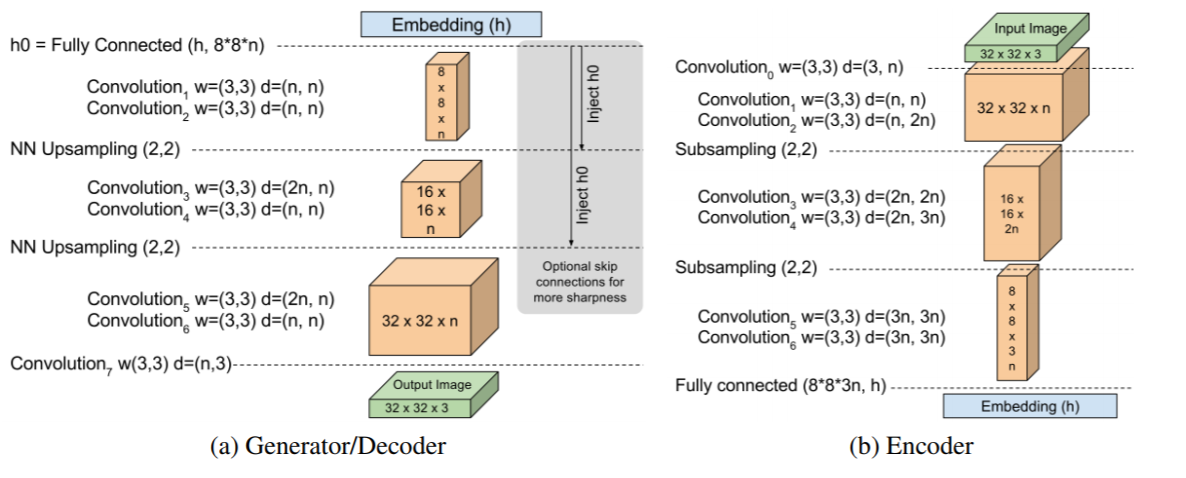
\includegraphics[width=4.0in]{BGAN_struct.png}
  \caption{BGAN的网络结构}
\end{figure}

\begin{figure}[!ht]
 \centering 
	\subfigure[1epoch]{
	\includegraphics[width=1.3in,height=1.3in]{BGAN1.png}
	}
	\subfigure[5epoch]{
	\includegraphics[width=1.3in,height=1.3in]{BGAN2.png}
	}
	\subfigure[10epoch]{
	\includegraphics[width=1.3in,height=1.3in]{BGAN3.png}
	}
	\subfigure[100epoch]{
	\includegraphics[width=1.3in,height=1.3in]{BGAN4.png}
	}
	\caption{人脸图片生成效果图}
\end{figure}
结果显示在人脸生成的过程之中,可以产生非常具有迷惑性和真实性的人脸,是对抗生成网络作为人脸生成的基石之一。但是在监督学习的框架之下,使用对抗生成生成训练数据还有关键的一步,就是如何获取生成样本的标签。虽然在上文提到的C对抗生成和Info对抗生成都有对于生成带有标注的人脸的尝试,但是从具体的效果中发现其效果还具有一定的不自然性,对于这种情况我们分析之后觉得没有尝试的必要,
\begin{figure}[h]
\centering
\subfigure[连续输入的对抗生成输出变化]{
\includegraphics[width=2.0in]{GAN-face-serilize.jpg}
}
\subfigure[随机输入的对抗生成输出变化]{
\includegraphics[width=2.0in]{GAN-face.jpg}
}
\subfigure[使用对抗生成网络生成戴眼镜的人脸	]{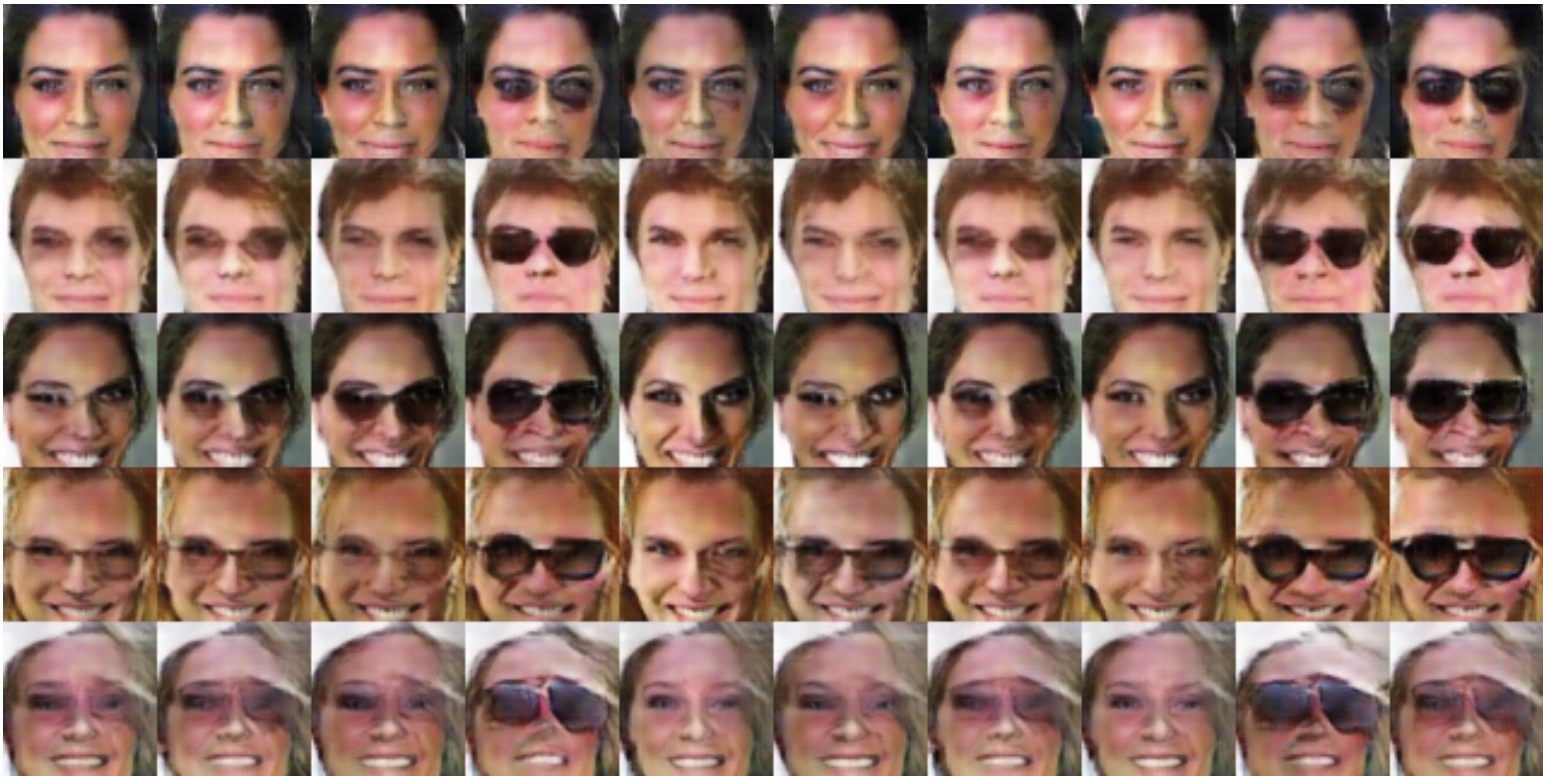
\includegraphics[width=5.0in]{infoGANglass.png}}
\caption{对抗生成网络生成图片的局限性}
\end{figure}

主要有以下几点原因:
.对抗生成网络的原理是拆解训练图片中的图像分布因子,将其储存在网络的参数之中,而随机噪声的输入,随着不断反卷积的操作,将输出的模式不断固化并且最终映射回原本的图像空间,其实是一个低维向高维投射的过程,但是因为投射的两维其实都是具有无限可能的,所以确实有完成这种也映射的可能,更何况人脸认为现实中存在的脸本身的范围就要比图像空间所能表示的范围要小得多。
但是基于目前CNN方法的对抗生成网络的原理是学习数据中的图像分布和梯度下降法的学习方法其实核心是针对于损失函数的优化,虽然在WGAN中对于对抗生成网络的损失函数又一次做出了优化,但依然不能够完美的和我们的任务相匹配,我们甚至不清楚自己想要的groundtruth是什么样的,所以损失函数的制定其实还不够出色,这也是为什么对抗生成网络的输出虽然显得很惊艳,但大多数时候还是会给人一种不真实感觉的原因。
所以在没有合格的损失函数之前,是不能够使用现有的对抗生成网络来进行神经网络的监督学习训练的,因为对抗生成网络生成的图片并不能真实的代表真实图片的分布。

但是在本论文的实验后期,我们想到了使用对抗生成网络来尝试迁移学习上的能力,其中使用了对抗生成网络在超分辨率上的应用。
\subsection{使用对抗生成网络提高人脸分辨率}
在发现对抗生成网络其实并不能直接从噪声生成具有一定训练意义的图片之后,我们并没有气馁。在参考了很多具有使用意义的对抗生成网络工作之后,决定从超像素的方向重新研究。超分辨率是通过硬件或软件的方法提高原有图像的分辨率的过程。在人脸超分辨率的之中,核心的思想就是在不改变人脸身份信息和属性信息的情况下,将人脸图像的更多细节还原出来。
\subsubsection{使用对抗生成网络生成高分辨率的图片}
在借鉴了了超分辨率的框架之后,设计了超分辨率神经网络框架是TRGAN\cite{TRGAN},
\begin{figure}[!ht]
\centering
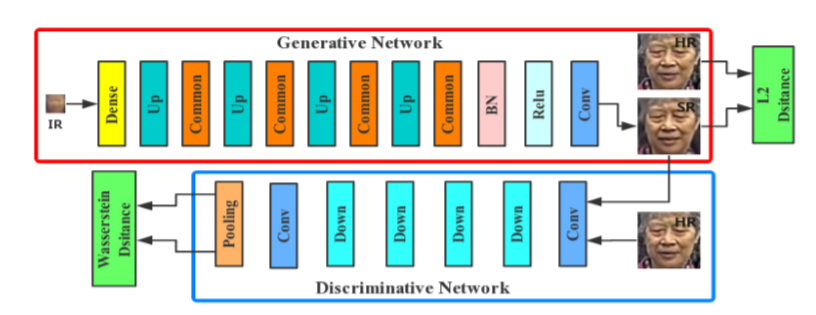
\includegraphics[width=6.0in]{TRGAN.png}
\caption{人脸超分辨率所使用的网络结构}
\end{figure}

具体来讲:
common模块:参考了resnet\cite{RESNET}的block模块,输入特征图分成两个分支,一个分支接BatchNorm之后接卷积层,再接一层batchnorm层和一层卷积层,最后该分支的block输出的特征图与另一个未经操作的分支使用元素对位相加(elementWise)。其目的是为了增加网络的深度,同时又能够为多层特征的融合提供不同的通道。

upSample模块:
在common模块的基础上,输入层的第一个分支连接到第一层卷积之后使用pixel shuffle\cite{ESPCN}的操作之后将图像尺寸变为原来的2倍。然后再接一层BatchNorm和卷积;
与此同时,第二层分支使用常规的双线性插值的方法扩大到两倍大小,使用1x1卷积连接之后将两个分支elementWise相加。
upsampling的操作相比common层的操作,可以让特征图变为原来的两倍大小,又增加了一定的特征融合。

downsample模块:
downsample的操作在common的基础上分别在两个分支的后面加入了stride为2的pooling层,可以保证输出特征图的大小为原来的一半。
\begin{figure}
\centering
\subfigure[Common模块]{
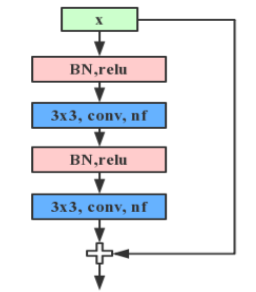
\includegraphics[width=1.50in]{a_common.png}
}
\subfigure[UpSample模块]{
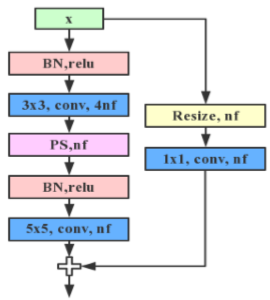
\includegraphics[width=1.50in]{b_up.png}
}
\subfigure[DownSample模块]{
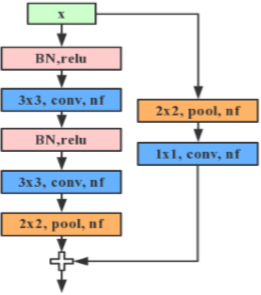
\includegraphics[width=1.50in]{c_down.png}
}
\caption{TRGAN中基于resnet的三种网络结构改进}
\end{figure}
使用该框架在celeA数据集上进行性训练,其中输入是8*8的低分辨率人脸,输出是64*64的高清人脸。优化的损失函数分别是输出的图片与原始高清图片的差值以及WGAN中的Wasseserstein Distance.
\begin{equation}{
W(P_r, P_g) = \frac{1}{K} \sup_{||f||_L \leq K} \mathbb{E}_{x \sim P_r} [f(x)] - \mathbb{E}_{x \sim P_g} [f(x)]
}
\end{equation}
具体的超分辨率实验结果:
\begin{figure}[!ht]
 \centering 
	\subfigure[像素为16*16的原图]{
	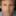
\includegraphics[width=0.25in,height=0.25in]{lr_Aaron_Eckhart_0001.jpg}
	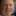
\includegraphics[width=0.25in,height=0.25in]{lr_Aaron_Guiel_0001.jpg}
	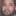
\includegraphics[width=0.25in,height=0.25in]{lr_Aaron_Patterson_0001.jpg}
	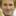
\includegraphics[width=0.25in,height=0.25in]{lr_Aaron_Peirsol_0001.jpg}
	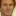
\includegraphics[width=0.25in,height=0.25in]{lr_Aaron_Peirsol_0002.jpg}
	}
	\subfigure[像素为64*64的原图]{
	
\includegraphics[width=1.0in,height=1.0in]{hr_Aaron_Eckhart_0001.jpg}
	
\includegraphics[width=1.0in,height=1.0in]{hr_Aaron_Guiel_0001.jpg}
	
\includegraphics[width=1.0in,height=1.0in]{hr_Aaron_Patterson_0001.jpg}
	
\includegraphics[width=1.0in,height=1.0in]{hr_Aaron_Peirsol_0001.jpg}
	
\includegraphics[width=1.0in,height=1.0in]{hr_Aaron_Peirsol_0002.jpg}
	}
	\subfigure[像素为64*64的超像素图]{
	
\includegraphics[width=1.0in,height=1.0in]{sr_Aaron_Eckhart_0001.jpg}
	
\includegraphics[width=1.0in,height=1.0in]{sr_Aaron_Guiel_0001.jpg}
	
\includegraphics[width=1.0in,height=1.0in]{sr_Aaron_Patterson_0001.jpg}
	
\includegraphics[width=1.0in,height=1.0in]{sr_Aaron_Peirsol_0001.jpg}
	
\includegraphics[width=1.0in,height=1.0in]{sr_Aaron_Peirsol_0002.jpg}
	}
	\caption{超分辨率使用lfw图片的效果示意图}
\end{figure}

可以看到对抗生成网络在超分辨率领域上取得了非常好的效果,可以在基本不改变人脸属性和身份信息的情况下,获取高清的图片。但是我们也发现一些有趣的现象:生成的图片虽然基本的轮廓不变,但是整体都相比原来更加白皙明亮了一些,整体给人的感觉都更加好看了一些。这其实是因为训练数据的图片都是celeA中的明星,其图片质量都比较出色,画风也带有一定的电影元素,似乎是把celeA的风格带到了lfw中,于是我有了一个大胆的想法。
\section{结合对抗生成超像素实现迁移学习}
\subsection{人脸属性的监督式学习困境}
首先引入一个经典的模式识别场景,泛化能力的问题:
在之前的工作种,经常可以发现一个经常出现的问题,使用MTL的人脸属性框架进行人脸属性识别的过程中,具同样40个属性标签的两个数据集lfwA和celeA,两个在各自数据集上训练之后的模型,在各自数据集上的准确率都很高,但是在对方的测试集效果都比较糟糕。

如何进行改善呢?我们针对于这种情况设计了这样的思路:
问题引出:对于相同的网络模型,使用相同的训练方法,在不同数据集中的训练之后,对自身数据集的测试集准确率要远远高于其他数据集的测试集。
问题分析:首先这不是一个过拟合问题,因为对于数据集中训练集和测试集的准确率较高,所以网络的训练没有问题。但是对于不同数据集的测试集准确率很低,所以推测问题的出现是因为数据的分布不同

尝试解决办法:首先我们先假定网络模型容量可以容纳两个数据的分布(数据的分布可能不满足线性加法,但是应该满足集合性合并不减的特性,所以假定两种数据的分布集合会比原来更大,所以对于网络容量的要求会更大),既然数据的分布不同,就应当减少数据分布对于模型训练带来的影响。

第一种方法就是将两个数据集合并训练,如果标签相同,那么可以简单的将两个数据集合并成一个数据集训练,也可以首先在一个数据集上份训练,再经过另一个数据集finetune,又或者采用上一章所提到的主干网路参数共享,不同数据集分别使用一个网络支线进行训练。都可以直观地学习到两个数据集之间的数据分布。往往就可以取得较好的效果,有效的提高在不同数据集上准确率的表现。

缺点:最致命的缺点就在于不同数据集的准确率提高,但是难以保证在自身的数据集上数据的准确性。即使采用较小的学习率谨慎的进行finetune,对于不同任务的训练过程也即将面临着大量的手动干预,还是处于一个监督学习的框架之中。

对此我们决定使用类似于迁移学习的方式来完成这个任务,并且结合对抗生成网络来完成我们的任务。
\subsection{人脸属性的迁移学习猜想}
迁移学习\cite{TRANSFER}是把一个领域(即源领域)的知识,迁移到另外一个领域(即目标领域),使得目标领域能够取得更好的学习效果。通常,源领域数据量充足,而目标领域数据量较小,迁移学习需要将在数据量充足的情况下学习到的知识,迁移到数据量小的新环境中。在图像领域,最主要完成迁移学习的方式就是将在源领域训练得到的模型作为特征提取器,然后在新的环境下使用诸如SVM、boosting等方式进行特征学习。或者固定模型的主要参数层,只重新训练后面针对于场景输出的特征提取类别。然后作为新环境的模型。

通常意义上的finetune,metric Learn ing也是迁移学习的分支。
而实际上迁移学习并没有明确的范围,其主要的目的是如何利用好已经学习到的知识,并将其应用到实际的应用场景之中。但实际场景虽然没有标注的数据,也是可以通过其他手段获取的知识,也就是说实际场景其实本身也是一种已经存在的知识,我们使用一些技巧将其已有的这是提取出来,并融合现有知识,完全有可能获得更加好的目标域识别效果。
\subsection{基于人脸超分辨率的人脸属性迁移学习实验}
在发现可以通过对抗生成网络将低分辨率人脸分辨率提高之后,我们设计了实验来针对上述问题进行研究。决定在lfwA的训练过程中混入超分辨率生成的LFWA人脸图像,目的也很明显,就是希望这些超分辨率的图片能够把celeA中的图像分布带到lfw中,从而提升使用lfwA数据训练的模型在在celeA数据上的性能。

实验中使用的网络是改进的alexnet主网络加上40个二分类的子网络模块。卷积层中的stride全部为1,保证网络特征图尺寸最后不会为消失。输入大小为64*64的人脸,通过上一章中提到的人脸矫正作为预处理的方式。使用人脸识别的与训练模型作为预训练基础。数据混合策略是按照将超像素图片和lfwA的原始图片按照1:1的比例作为训练数据。

实验结果如下:
\begin{table}[!h]
  \centering
   \caption{在CELEA数据集}
   \begin{tabular}{c|c|c}
     \toprule
     数据集训练 &数据集测试 &40属性平均准确率(\%)\\
     \midrule
      LFWA   &  CeleA &  66.2 \\
	  CeleA  &  CeleA &  89.1 \\
	  LFW-hr &  CeleA &  76.2 \\
      LFWA   &  LFWA  &  83.4 \\
	  CeleA  &  LFWA  &  70.7 \\
	  LFW-hr &  LFWA  &  83.3 \\
     \bottomrule
   \end{tabular}
\end{table}
\section{实验结果分析与结论}
从训练的结果来看可以看出,使用celeA训练数据的模型,在celeA测试集中取得了89.1\%的准确率,但是在lfwA上的准确率就降低了和蒂诺。只有70.7\%。类似的使用lfwA数据进行训练,也具有同样的现象。这符合人脸属性种监督学习的困境。
再加入了人脸超分辨率像素的进行训练之后,情况有了改善,不仅使用超分辨率像素训练的模型在原本的lfwA数据集上具有良好的效果,只是下降了0.1个百分点,在celeA数据集上也提升10个百分点。这说明基于超分辨率的像素来完成人脸属性识别是可行的。通过改变训练数据的情况下,对数据的预处理过程添加了一定其他环境噪声分布,这和传统通过数据增强的方式完成的数据噪声加入是有很大不同的。原始的数据增强例如平移、旋转、色彩通道等变换等都还是对于现有数据分布从离散化的输入到连续化扩充,是可以充分的利用输入数据的分布资源。但超分辨的图像变换形式其实可以更深层次的改变图像的状态而最大限度保留图像的标注信息不发生改变。这样是最直接的增加数据分布的方式。尤其是在本实验中lfwA中的图片数量较少,数据的分布也更加偏僻且具有离散化,和celeA也有很大的差距,简单的数据增强其实并不能完全解决这个问题。所以使用超分辨率的方式进行扩充训练可以取得更好的效果。

但是不得不承认,虽然本文中没有常熟将celeA和lfwA数据进行混合训练的方式,但是无疑这样的方式其实最直接提升在不同数据场景下识别效果的方式,而且流程更加简单,使用训练数据并行的训练方式其实是可以取得优异的效果的。然而基于超分辨率的迁移学习的优势其实体现在对于未知数据场景的学习能力。在现有数据中进行模型的学习,然后针对于不同的数据场景,使用超分辨率的模型对于场景图片进行学习和复现,这样可以轻松从有标注的数据的低分辨率版本获得有标注数据在对应场景的移植高分辨率版。再将移植的高分辨率的图像通过正常训练的图片。

\section{本章小结}
在本章中首先对于对抗生成网络的相关技术做了介绍,然后研究了对抗生成网络现实中比较常见的应用包括使用对抗生成网络生成真实图像和使用对抗生成网络提高图片的分辨率。在探究和实验的过程之中,我们完成了相关的图片生成任务,g对抗生成网络也体现出了非常令人眼前一亮的伪造图片能力。但针对于人脸属性任务对于图片的要求,生成图片依然很难满足相关的真实程度和标签要求。

但是使用超分辨率对于低分辨率人脸的修复和生成体现了良好的效果。于是结合迁移学习的方式,我们对于人脸属性识别在不同场景的识别效果做了探究性实验。
总结来说,迁移学习是监督学习之后最具有研究方向的领域,我们对此进行探究,并发现在我们固定的实验方法和celeA与lfwA 40种属性分类的场景下,使用基于超分辨率的学习方法确实可以有一定的效果提升。